\documentclass[a4paper]{article}
\usepackage[utf8]{inputenc}
\usepackage{fullpage}
\usepackage{csquotes}
\usepackage[ngerman]{babel}
\usepackage{biblatex}
\usepackage{float}
\usepackage{graphicx}
\usepackage{listings}
\bibliography{documentation}
\usepackage{listings}
\usepackage{minted}
\usemintedstyle{default}
\title{PowPow Dokumention}
\author{Willi Schönborn}
\date{\today}
\begin{document}

\maketitle

\newpage
\tableofcontents

\newpage
\section{Einleitung}

\subsection{Aufgabenstellung}
Idee + Gerüst + Prototyp + Dokumentation

\subsection{Idee}
\begin{figure}[H]
\centering
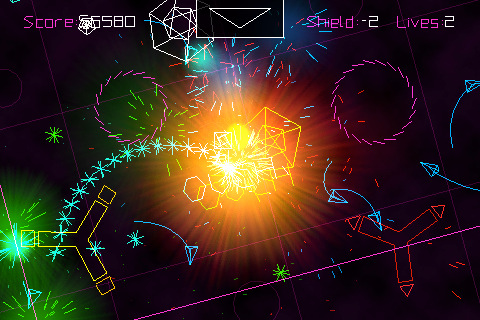
\includegraphics[width=0.7\textwidth]{PewPew-iPhone-App-Review.jpg}
\caption{PewPew}
\end{figure}

\newpage
\section{Implementierung}

\subsection{Scala}

\subsection{Architektur}
\inputminted[firstline=20, lastline=36]{scala}{../scala/org/whiskeysierra/powpow/Ship.scala}
\subsection{Bulletphysics}
\subsection{Jinput}
\subsection{Shaders}

\newpage
\section{Fazit}

\begin{figure}[H]
\centering
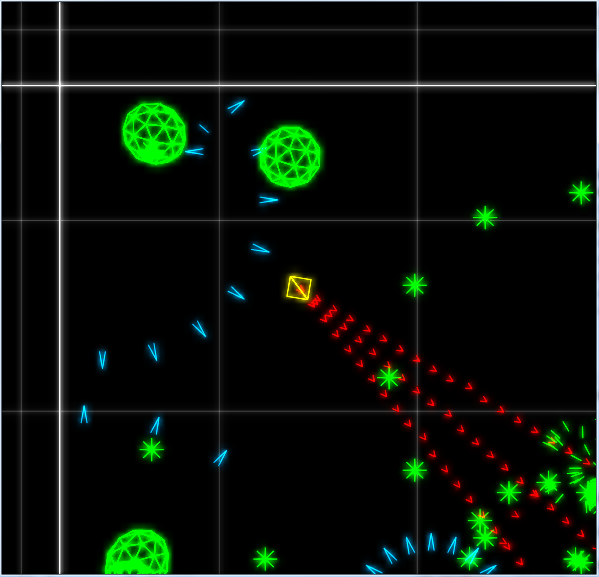
\includegraphics[width=0.7\textwidth]{screenshot1.png}
\caption{In-Game Screenshot}
\end{figure}

\begin{figure}[H]
\centering
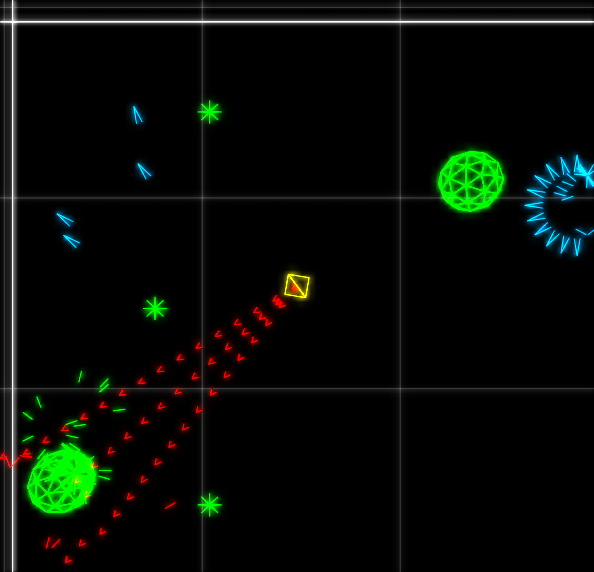
\includegraphics[width=0.7\textwidth]{screenshot2.png}
\caption{In-Game Screenshot}
\end{figure}

\newpage
\nocite{pewpewgame}
\nocite{jinput}
\renewcommand{\refname}{Quellen}
\addcontentsline{toc}{section}{Quellen}
\printbibliography

\addcontentsline{toc}{section}{Abbildungsverzeichnis}
\listoffigures

\end{document}

